

\section{Introduction}


Video inpainting aims to recover the missing contents of given videos, which can assist lots of practical applications, e.g., video restoration and augmented reality. Compared with image inpainting, video inpainting is much more challenging due to the extra time dimension. It requires not only reasonable spatial structures but also temporal consistency. 
Though great progress has been made in 2D image inpainting using deep learning techniques \cite{yu2018free,Xiong_2019_CVPR}, directly applying these approaches to each individual frame in video inpainting could lead to artifacts, flickers and jitters. 

\begin{figure}[t]
	\centering
	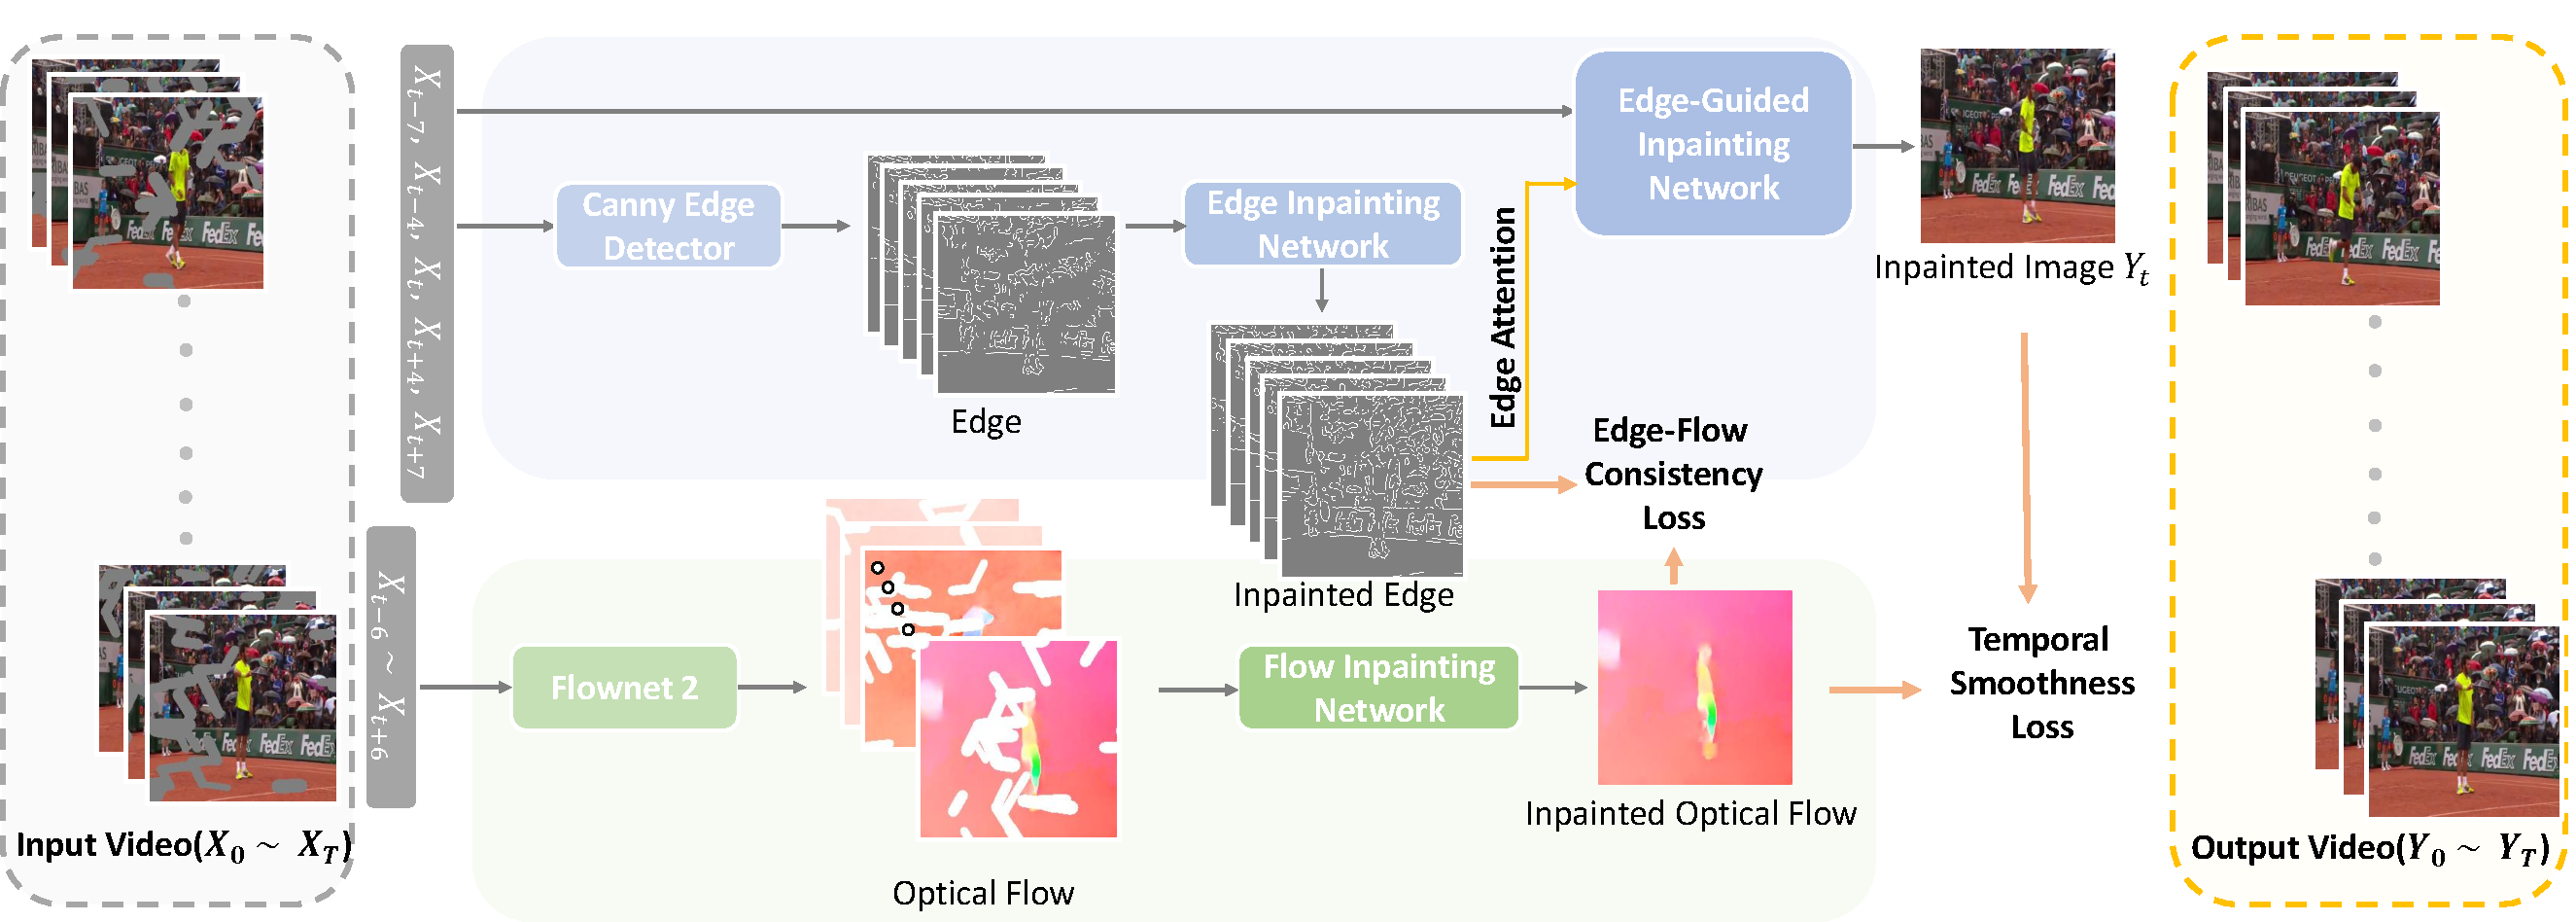
\includegraphics[width=1.0\columnwidth]{zong} % Reduce the figure size so that it is slightly narrower than the column. Don't use precise values for figure width.This setup will avoid overfull boxes. 
	\caption{The overall pipeline of SOVI. The ENet first completes the missing edge across frames. Then, under the guidance of structural edge, TINet can produce structure-preserved inpainting frame. Moreover, the FNet is designed to predict missing optical flow, which provides temporally consistency to the final result.}
	\label{zong}
\end{figure}


To exploit complementary information across neighboring frames, traditional patch-based methods \cite{patwardhan2007video,wexler2004space,newson2014video} recurrently copy similar patches from unmasked regions and past them to the missing regions. 
This kind of method depends on a strong hypothesis that the missing content have precisely appeared in neighboring frames, which limits their generalization.
Recently, deep-learning based methods achieve state-of-the-art performance by treating a video as a 3D volume.
They utilize 3D convolution layers to predict missing content with smooth motion \cite{wang2019video}.
Among these methods, optical flow is commonly used to temporally smooth the inpainted contents \cite{Xu_2019_CVPR,Kim_2019_CVPR,Kim_2019_CVPR1} by aggregating the contextual information from neighboring frames.
By introducing motion knowledge, the above methods give promising inpainting results with temporal consistence.
However, structural  rationality is also a significant factor for realistic video inpainting. Existing methods implicitly learn to reconstruct structure during texture generation, which tend to generate over-smoothed regions. 
Similar observations are obtained in image inpainting \cite{Xiong_2019_CVPR,nazeri2019edgeconnect}. %\cite{iizuka2017globally,liu2018partialinpainting,yu2018free}. 
To solve this problem, they propose to predict object contours or edges as auxiliary information.
Despite structure-preserved image inpainting, it remains an open problem of how to simultaneously explore the structure and motion information in videos.
%However, when it comes to videos, 
%it is non-trivial to manage correlation between edge, motion and texture inpainting.
%applying image inpainting methods in a frame-by-frame manner will cause serious flickering artifacts. Besides, the problem of how to utilize structure information in video inpainting effectively is also non trivial.
%just  learned with texture and flow generation by existing methods.
%Thus, how to obtain fine-detailed inpainting video remains an open problem.
%is hard to capture the detailed information accurately. 

%has been proven to generate over-smoothed regions in \cite{nazeri2019edgeconnect}
%Besides, complementary information brought by optical flow also lacks structure guidance when the contents are missed in neighboring frames.








In this paper, we present a novel structure-oriented video inpainting network (SOVI) that can collect and exploit the structure information to improve video inpainting results. %SOVI extracts fine-detailed structure and the information
The key insight of SOVI is to explore the correlation among structure, motion, and texture for simultaneously fine-detailed and temporal coherent video generation. %This is significant departure from existing works [], where the texture is only associated with motion or structure.
%We  predict the edges, which well represents structure information. To embed  
%\cxj{Explain more about the concept. not the modules.}
As shown in Fig.~\ref{zong}, our method consists of three modules, which are respectively the edge inpainting network (ENet), flow inpainting network (FNet), and texture inpainting network (TINet).
Given frames with missing pixels, ENet first completes the edge maps that indicate the detailed structure information. Then, under the guidance of completed edge, TINet is developed to fill the missing colors and textures in a coarse-to-fine manner.
Specifically, a structure attention module is designed to capture the latent spatial relevance between video textures and structure edges.
Compared with original edge maps, the structure-texture relevance is easier to be embedded into TINet, which benefits fine-detailed frame generation.
Besides, the developed FNet can predict the missing optical flow, which provides auxiliary motion knowledge. Explicitly, a flow-edge consistency constraint and a temporal ensemble module are utilized to smoothen the edge maps and final inpainted frames, based on the motion tendency. Consequently, the inpainted frames by SOVI are not only detail-preserved but also temporal consistent.
%\cxj{This is about 'how', not about 'why'.}
%by simultaneously exploring optical flow and , to eliminate temporal flickers and enhance spatial detail. 
%  and FNet  and optical flow,  knowledge and motion tendency.
%according to learned structure knowledge and motion tendency from the training data,
%Instead of separate training, these two modules are
%This results in both edge-enhanced optical flow and temporally smooth edge. 
%Specifically, a structure enhancement mechanism is developed to extract and refine the structural clues in the completed edge and encode them into the STI.
% the optical flow is used by propagating complementary pixels from neighboring frames to current frame to alleviate artificial flickers and jitters.


%In summary, we present a novel structure-oriented video inpainting method, which can generate structural reasonable and temporal coherent inpainted frames.
%
Experiments on YouTubeVOS and DAVIS datasets show that the proposed method obtains new state-of-the-art performance with low time consumption, which demonstrates its superiority.
%
Our contributions can be summarized as follows:
\begin{itemize}
	\item We propose a novel structure-oriented video inpainting method, which combines edge completion, motion generation, and video inpainting for simultaneous fine-details and temporal consistency.
	\item A novel structure attention module is designed to capture the spatial relevance between video contents and structure edges, which is easily to be embedded into video inpainting network. %With edge collection and structure embedding, we demonstrate the significance of detailed structure in video inpainting. 
	%to structure information is well represented and encoded in video inpainting via . 
	\item A flow-guided warping and temporal ensemble module are developed to enhance temporal consistency for video inpainting.%, with a flow inpainting network.
	%	Optical flow is used to enhance temporal consistency, which 
	
	
	%	We propose a novel structure- for video inpainting, by simultaneously exploring optical flow and structural clues to eliminate temporal flickers and enhance structure detail. 
	%	 A flow-edge consistency loss is developed to associate the optical flow and structure edges, which can boost each other.
	%	\item  a structure enhancement mechanism is  designed, which can promote the video inpainting.	
	
\end{itemize}





\section{Related Work}
\subsubsection{Traditional Image/Video Inpainting.}
Traditional image and video inpainting methods can be divided into two categories, diffusion-based and patch-based methods. 
Diffusion-based methods \cite{bertalmio2000image,ballester2001filling} gradually propagate contents from surrounding areas to the missing regions. 
However, this kind of method fails to handle large holes due to error accumulation. 
Patch-based methods~\cite{bertalmio2003simultaneous,efros2001image} formulate the completion task as a patch-based optimization problem, which is more widely used. 
It fills the missing image contents by borrowing and aggregating the most similar patches from known regions. 
\cite{patwardhan2007video} further extends the task to video inpainting by searching patches in across frames. \cite{newson2014video} enhances the quality of video inpainting by using a video version of PatchMatch algorithm \cite{barnes2009patchmatch}. 
Then, \cite{huang2016temporally} proposes completing the missing optical flow to alleviate the temporal artifacts and enforce temporal consistency. 
However, traditional methods assume that there should exist complementary contents in known regions, which can not synthesize unseen appearances. Besides, the propagation process makes these methods suffer from high computational complexity, which limits their usage in practical applications. 

\subsubsection{CNN-based Image/Video Inpainting.}
Recently, deep learning methods  have achieved tremendous progress because of their capability of capturing high-level semantic information of images and videos. 
first introduces 
The convolution neural network (CNN) is first introduced to synthesize small unknown regions and denoise in images \cite{xie2012image}. 
To improve the photorealism of the completed results, a generative adversarial network is employed \cite{pathak2016context} by jointly training a generator and a discriminator in a minimax manner. 
Then, \cite{iizuka2017globally} proposes using two discriminators to constrain both global and local coherence of image contents. Later, \cite{liu2018partialinpainting} designs partial convolution to handle holes of irregular shapes. \cite{yu2018free} introduces gated convolution to learn a dynamic feature selection mechanism in CNN.
%However, methods aforementioned usually handle the square masks, which produce artificial when recovering challenging holes of irregular shapes. 
%\cxj{What is the underlying difference between these two mask shapes?}
%
%%% irregular  masks
%To solve this,
%. Later, \cite{yu2018free} introduces gated convolution to learn a dynamic feature selection mechanism in CNN.  
\cite{nazeri2019edgeconnect} introduces an edge generator to refine generated structure in image inpainting. These image inpainting methods can obtain plausible synthesized images. 
%\cxj{In comparison, what is the difference of our method when sovling irregular masks?}


%%% video inpainting 
However, directly extending these state-of-the-art image inpainting methods to video domain is not an optimal solution, which will generate videos with serious temporal flickers, artifacts and jitters. Besides, Image inpainting methods can not utilize useful complementary information in neighboring frames. To obtain spatio-temporal consistent inpainted video, some methods have been proposed recently.
\cite{wang2019video} proposes CombCN to capture both temporal and spatial consistency, which is the first to use CNN-based method in video inpainting. \cite{Xu_2019_CVPR} proposes a stacked convolution network to predict missing motion field and regards video inpainting as a pixel propagation problem. \cite{Kim_2019_CVPR} automatically removes texts in videos without mask indications, which aggregates temporal features from encoder to decoder and applies a recurrent feedback. \cite{Kim_2019_CVPR1} introduces convolutional LSTM and temporal feature aggregation to obtain temporal consistency and learn information from neighboring frames. However, these existing methods neglect the importance of structure information in video inpainting, which will cause the blurry details and structural cracks in generated videos. 

Different from the methods above, SOVI extract and refine structure information explicitly, which will generate fine-detailed video inpainting results.
%predict edge maps explicitly, which well represent structure details. 
%\cxj{What is our key difference?}


\dlt{
	To tackle these issues, we propose a novel structure-oriented video inpainting network (SOVI) based on CNN.
	Different from the methods above, SOVI
	takes the effect of structure information into consideration. In our network, we collect and refine the structure information to enhance the final generated video. Specifically, a structure attention module is introduced to learn latent correlation between video contents and structure. Besides, temporal consistency is also guaranteed through flow-guided warping and temporal ensemble module. Finally, we can generate spatio-temporal consistent inpainted video. 
}






























%\section{Introduction}
%
%
%Video inpainting aims to recover the missing contents of given videos, which can assist lots of practical applications, e.g., video restoration and augmented reality. The task requires not only reasonable spatial structures but also temporal consistency. 
%
%Existing video inpainting methods exploit structural information by propagating complementary information across neighboring frames implicitly. \cite{patwardhan2007video,wexler2004space,newson2014video} recurrently copy similar patches from unmasked regions and past them to the missing regions. This kind of method depends on a strong hypothesis that the missing contents have precisely appeared in neighboring frames, which limits their generalization. Recently, deep-learning based methods achieve state-of-the-art performance by treating a video as a 3D volume. They utilize 3D convolution layers to predict video frames \cite{wang2019video}. Among these methods, optical flow is commonly used to propagate appearances by aggregating the contextual information from neighboring frames \cite{Xu_2019_CVPR,Kim_2019_CVPR,Kim_2019_CVPR1}.
%However, the missing structural details can not be created by motion compensation. 
%Thus, the auxiliary information brought by optical flow lacks detailed structural clues, e.g. the inner textures of objects are usually missed in flow field, leading to deficient structure rationality and video blurs.
%
%Image inpainting methods \cite{Xiong_2019_CVPR,nazeri2019edgeconnect} predict object contours or edges for structure enhancement. Though these methods can obtain sharp-detailed images to some degrees, directly applying these approaches to each individual frame in video inpainting will lead to serious artifacts, flickers and jitters.  Thus, how to obtain fine-detailed inpainting video remains an open problem.
%%Compared with image inpainting, video inpainting is much more challenging due to the extra time dimension. 
%%\mdf{Though great progress has been made in 2D image inpainting using deep learning techniques \cite{yu2018free,Xiong_2019_CVPR}, directly applying these approaches to each individual frame in video inpainting could lead to artifacts, flickers and jitters. }
%
%In this paper, we present a novel structure-oriented video inpainting network (SOVI) that can collect and refine the structure information to improve the inpainting results. 
%The proposed SOVI is based a 3-node graph of motion, structure, and texture. This is based on the key insight that the structure and motion are two significant factors for a realistic video content. This is significant departure from existing works \, where the texture is only associated with motion or structure.
%
%%To exploit complementary information across neighboring frames, traditional patch-based methods \cite{patwardhan2007video,wexler2004space,newson2014video} recurrently copy similar patches from unmasked regions and past them to the missing regions. 
%%This kind of method depends on a strong hypothesis that the missing content have precisely appeared in neighboring frames, which limits their generalization.
%Recently, deep-learning based methods achieve state-of-the-art performance by treating a video as a 3D volume.
%%They utilize 3D convolution layers to predict missing content with smooth motion \cite{wang2019video}.
%%Among these methods, optical flow is commonly used to temporally smooth the inpainted contents \cite{Xu_2019_CVPR,Kim_2019_CVPR,Kim_2019_CVPR1} by aggregating the contextual information from neighboring frames.
%%However, the auxiliary motion compensation brought by optical flow lacks detailed structural clues, e.g. the inner textures of objects are usually missed in flow field, leading to deficient structure rationality.
%%\cxj{It is not clear why motion compensation lacks structural clues..}
%Thus, how to obtain fine-detailed inpainting video remains an open problem.
%
%
%
%
%\begin{figure}[t]
%	\centering
%	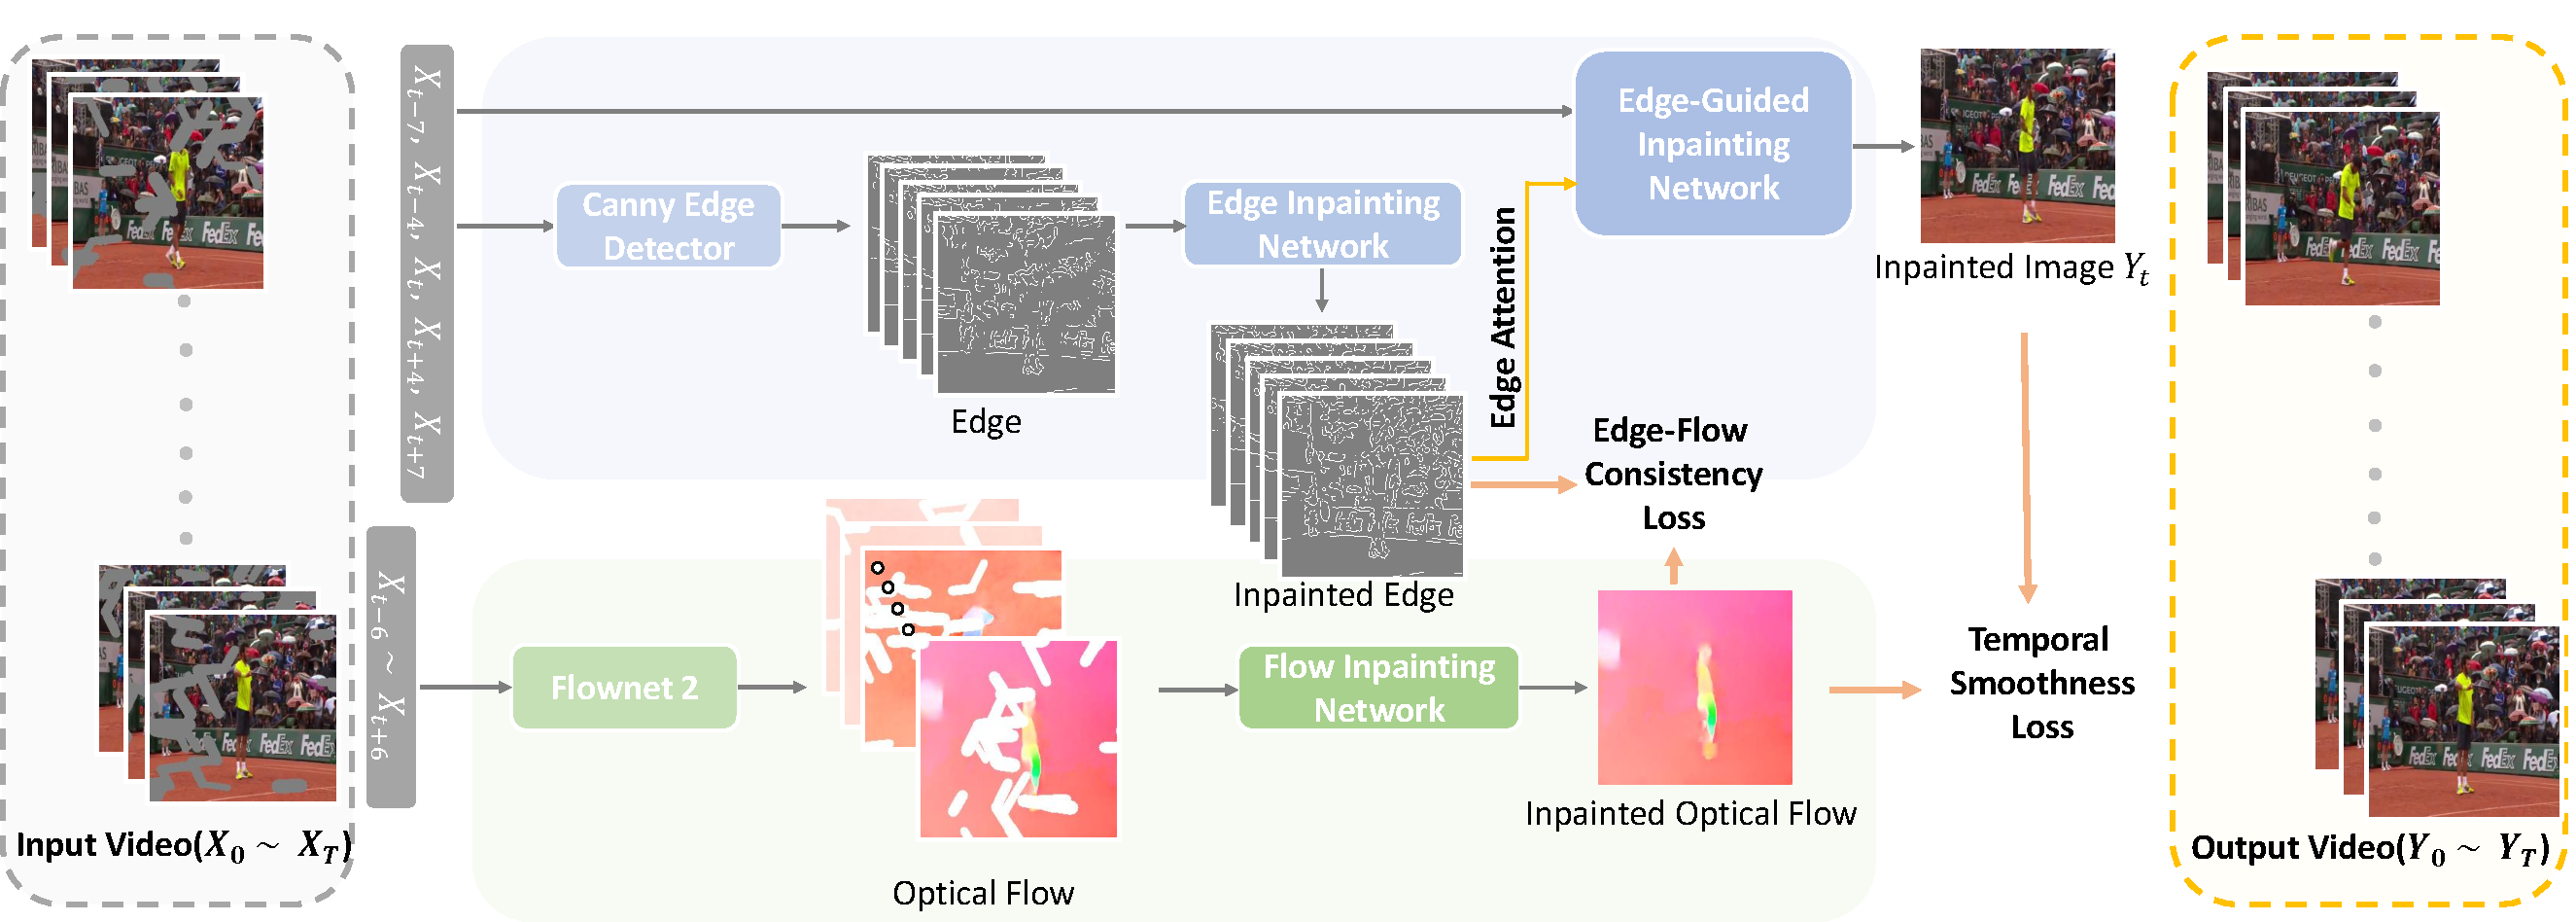
\includegraphics[width=1.0\columnwidth]{zong} % Reduce the figure size so that it is slightly narrower than the column. Don't use precise values for figure width.This setup will avoid overfull boxes. 
%	\caption{The overall pipeline of SOVI. The ENet first completes the missing edge across frames. Then, under the guidance of structural edge, TINet can produce structure-preserved inpainting frame. Moreover, the FNet is designed to predict missing optical flow, which provides temporally consistency to the final result.}
%	\label{zong}
%\end{figure}
%
%
%In this paper, we present a novel structure-oriented video inpainting network (SOVI) that can collect and refine the structure information to improve the inpainting results. 
%\cxj{Explain more about the concept. not the modules.}
%As shown in Fig.~\ref{zong}, our method consists of three modules, which are respectively the edge inpainting network (ENet), flow inpainting network (FNet), and spatio-temporal inpainting network (TINet).
%Given frames with missing pixels, ENet first completes the edge maps that indicate the detailed structure information. Then, under the guidance of completed edge, TINet is developed to fill the missing colors and textures in a coarse-to-fine manner.
%Specifically, a structure attention module is designed to capture the latent spatial relevance between video contents and structure edges.
%Compared with original edge maps, the structure-texture relevance is easier to be embedded into TINet, which benefits fine-detailed frames generation.
%Besides, the developed FNet can predict the missing optical flow, which provides auxiliary motion knowledge. Explicitly, a flow-edge consistency constraint and a temporal ensemble module are utilized to smoothen the edge maps and final inpainted frames, based on the motion tendency. Consequently, the inpainted frames by SOVI are not only detail-preserved but also temporal consistent.
%\cxj{This is about 'how', not about 'why'.}
%%by simultaneously exploring optical flow and , to eliminate temporal flickers and enhance spatial detail. 
%%  and FNet  and optical flow,  knowledge and motion tendency.
%%according to learned structure knowledge and motion tendency from the training data,
%%Instead of separate training, these two modules are
%%This results in both edge-enhanced optical flow and temporally smooth edge. 
%%Specifically, a structure enhancement mechanism is developed to extract and refine the structural clues in the completed edge and encode them into the STI.
%% the optical flow is used by propagating complementary pixels from neighboring frames to current frame to alleviate artificial flickers and jitters.
%
%
%In summary, we present a novel structure-oriented video inpainting method, which can generate structural reasonable and temporal coherent inpainted frames.
%%
%Experiments on YouTubeVOS and DAVIS datasets show that the proposed method obtains new state-of-the-art performance with low time consumption, which demonstrates its superiority.
%%
%This improvement derives from two technical contributions:
%\begin{itemize}
%
%\item We introduce an edge inpainting network to predict the missing edges. Besides, a novel structure attention module is designed to capture the spatial relevance between video contents and structure edges, which is easily to be embedded into video inpainting network. %With edge collection and structure embedding, we demonstrate the significance of detailed structure in video inpainting. 
%	%to structure information is well represented and encoded in video inpainting via . 
%\item A flow-guided warping and temporal ensemble module are developed to enhance temporal consistency for video inpainting, with a flow inpainting network.
%	%	Optical flow is used to enhance temporal consistency, which 
%
%	
%	%	We propose a novel structure- for video inpainting, by simultaneously exploring optical flow and structural clues to eliminate temporal flickers and enhance structure detail. 
%	%	 A flow-edge consistency loss is developed to associate the optical flow and structure edges, which can boost each other.
%	%	\item  a structure enhancement mechanism is  designed, which can promote the video inpainting.	
%	
%\end{itemize}
%
%
%
%
%
%\section{Related Work}
%\subsubsection{Traditional Image/Video Inpainting.}
%Traditional image and video inpainting methods can be divided into two categories, diffusion-based and patch-based methods. 
%Diffusion-based methods \cite{bertalmio2000image,ballester2001filling} gradually propagate contents from surrounding areas to the missing regions. 
%However, this kind of method fails to handle large holes due to error accumulation. 
%Patch-based methods~\cite{bertalmio2003simultaneous,efros2001image} formulate the completion task as a patch-based optimization problem, which is more widely used. 
%It fills the missing image contents by borrowing and aggregating the most similar patches from known regions. 
%\cite{patwardhan2007video} further extends the task to video inpainting by searching patches in across frames. \cite{newson2014video} enhances the quality of video inpainting by using a video version of PatchMatch algorithm \cite{barnes2009patchmatch}. 
%Then, \cite{huang2016temporally} proposes completing the missing optical flow to alleviate the temporal artifacts and enforce temporal consistency. 
%However, traditional methods assume that there should exist complementary contents in known regions, which can not synthesize unseen appearances. Besides, the propagation process makes these methods suffer from high computational complexity, which limits their usage in practical applications. 
%
%\subsubsection{CNN-based Image/Video Inpainting.}
%Recently, deep learning methods  have achieved tremendous progress because of their capability of capturing high-level semantic information of images and videos. 
%% first introduces 
%The convolution neural network (CNN) is first introduced to synthesize small unknown regions and denoise in images \cite{xie2012image}. 
%To improve the photorealism of the completed results, a generative adversarial network is employed \cite{pathak2016context} by jointly training a generator and a discriminator in a minimax manner. 
%Then, \cite{iizuka2017globally} proposes using two discriminators to constrain both global and local coherence of image contents. 
%However, methods aforementioned usually handle the square masks, which produce artificial when recovering challenging holes of irregular shapes.
%\cxj{What is the underlying difference between these two mask shapes?}
%%
%
%%%% irregular  masks
%To solve this,
% \cite{liu2018partialinpainting} designs a network which utilizes the partial convolution. Later, \cite{yu2018free} introduces gated convolution to learn a dynamic feature selection mechanism in CNN.  \cite{nazeri2019edgeconnect} introduces an edge generator to refine generated structure in image inpainting. These image inpainting methods can obtain plausible synthesized images. 
%\cxj{In comparison, what is the difference of our method when sovling irregular masks?}
% 
%
%%%% video inpainting 
% However, directly extending these state-of-the-art image inpainting methods to video domain is not an optimal solution, which will generate videos with serious temporal flickers, artifacts and jitters. Besides, image inpainting methods can not utilize useful complementary information in neighboring frames. To obtain spatio-temporal consistent inpainted video, some methods have been proposed recently.
%\cite{wang2019video} proposes CombCN to capture both temporal and spatial consistency, which is the first to use CNN-based method in video inpainting. \cite{Xu_2019_CVPR} proposes a stacked convolution network to predict missing motion field and regards video inpainting as a pixel propagation problem. \cite{Kim_2019_CVPR} automatically removes texts in videos without mask indications, which aggregates temporal features from encoder to decoder and applies a recurrent feedback. \cite{Kim_2019_CVPR1} introduces convolutional LSTM and temporal feature aggregation to obtain temporal consistency and learn information from neighboring frames. However, these existing methods neglect the importance of structure information in video inpainting, which will cause the blurry details and structural cracks in generated videos. 
%\cxj{What is our key difference?}
%
%
%
%\dlt{
%To tackle these issues, we propose a novel structure-oriented video inpainting network (SOVI) based on CNN.
% Different from the methods above, SOVI
%takes the effect of structure information into consideration. In our network, we collect and refine the structure information to enhance the final generated video. Specifically, a structure attention module is introduced to learn latent correlation between video contents and structure. Besides, temporal consistency is also guaranteed through flow-guided warping and temporal ensemble module. Finally, we can generate spatio-temporal consistent inpainted video. 
%}